\section{Performance Assessment}
%

The performance of the proposed method is assessed by comparing its results to those of a commercially available state-of-the-art software package. Performance is measured quantitatively for canonical image masks defined by spheres of various radii and locations, and qualitatively using a variety of real MRI and CT scans. \\ \\
%
We pursue a quantitative understanding of the performance of our method by considering a sphere of radius $R$ and center $\bm{C}$.  We assign a material identifier $m$ to each voxel in the image to define our spherical image mask; for the voxel with center at $\bm{v}$, the material assignment is:
\begin{align} 
	m &=  \begin{cases}
		1, & \text{if}\ d \left(\bm{v},\bm{C}\right) \le R \\
		0, & \text{otherwise},
	\end{cases}
\end{align}
where $d(\cdot,\cdot)$ is the Euclidean distance. The background image is assumed to have a 256 $\times$ 256 $\times$ 256 voxel resolution.
%%%%%%%%%%%%%%%%%%%%%%%%%%%%%%%%%%%%%%%%%%%%%%%
%%%%%%%%%%%%%%%%%%%%%%%%%%%%%%%%%%%%%%%%%%%%%%%
\subsection{\textcolor{purple}{Error Measures}}
\label{Error Measures}

In order to quantify performance, two error metrics are defined: a {\em shape error} and a {\em volume error}. These metrics characterize the departure of the b-rep from the perfect sphere.  There are two sources of error~\cite{young_2008}: 1) error due to approximating the perfect sphere with a binary image mask, or the {\em image-based error}; and 2) error due to reconstructing the binary image mask with a facetized b-rep.  The latter dictates a method's ability to {\em converge to geometry}. The image mask defined above does not, of course, yield perfect image-based accuracy. For these purposes, though, we will assume that the image-based error is negligible, and we will focus on the ability of the method to converge to geometry.\\ \\
%
The shape error measures the surface-normal deviation of our algorithm's end-result b-rep from the perfect sphere. The measure is constructed first by projecting each facet of the b-rep onto the exact sphere. The normal of each facet is compared to the normal of the exact sphere at the centroid of the projected facet by computing the magnitude of their cross product. An area-weighted sum is then taken over the b-rep, and finally the sum is normalized by the surface area of the b-rep. The error measure therefore lies in the range $\left [0,1\right]$. The shape error $e_s$, as described, can be calculated from:
\begin{equation} 
	e_s = \frac{ \sum \limits_{f\in\mathcal{F}} A_f \lVert {\bf n}_f \times {\bf n}_s \rVert}{\sum \limits_{f\in\mathcal{F}} A_f},
\end{equation}
where $A_f$ is the area and ${\bm n}_f$ is the unit normal of facet $f$, $\mathcal{F}$ is the set of all b-rep facets, and ${\bm n}_s$ is the normal of the exact sphere at the centroid of the projected facet onto the sphere. \\ \\
%
The volume error measures the unsigned volume enclosed between the b-rep and the exact sphere. We calculate this measure via a sum of integrals over the projections $\gamma_f$ of each facet onto the exact sphere: 
\begin{equation}
\label{vol err}
	e_v = \frac{1}{4\pi R^2} \Big[\sum \limits_{f \in \mathcal{F}\textsl{}} \ \int \limits_{\gamma_f} (r - R)^2 d\alpha \Big]^{1/2} .
\end{equation}
Here, $r = \lVert {\bm x} \rVert$ is the distance from the sphere center to a point on the planar facet associated with the projection $\gamma_f$, and $R$ is the radius of the exact sphere.  The indicated integrals are performed numerically on the projected facets. Six quadrature points were found to provide sufficient accuracy. The volume error is rendered dimensionless by normalizing by the surface area of the underlying perfect sphere.
%%%%%%%%%%%%%%%%%%%%%%%%%%%%%%%%%%%%%%%%%%%%%%%
%%%%%%%%%%%%%%%%%%%%%%%%%%%%%%%%%%%%%%%%%%%%%%%
\subsection{\textcolor{purple}{The Unpolluted Sphere}}
\label{The Unpolluted Sphere}

The shape and volume errors were compared between the commercial software and the proposed method for a perfect sphere embedded in a fixed $256 \times 256 \times 256$ array of voxels.  In the comparisons presented below, three independent parameters were varied:  1) b-rep resolution, 2) sphere radius, and 3) sphere center location relative to the voxel array. The purpose of these comparisons is to show that the method performs comparably to an established option, rather than specifically pointing to the superiority of one method over the other. Optimal results were obtained from the commercial package by selecting the ``binarise before smoothing" option and performing 100 iterations of ``smart mask smoothing''; standard options were chosen otherwise. \\ \\
%
\figref{graph1} shows the shape and volume errors of the two methods as the b-rep resolution is varied for a spherical mask centered in the image with radius $R = 80$ voxels. See~\figref{demos1} for a visual comparison of the image mask with representative b-reps from the commercial code and the proposed method. Default parameters were used in the commercial code for b-reps with $n \ge 2587$ vertices. For resolutions coarser than that, the ``target maximum error" was increased to allow results with $n < 2587$. When comparing the shape error of the two approaches, the proposed method performs at least as well as the commercial option for coarse meshes ($n < 2500$), while it performs measurably better -- up to $40\%$ improvement -- for finer b-reps ($n > 5000$). For the volume error, the proposed method performs up to $70\%$ better for b-reps with resolutions of $n < 5000$ vertices, and converges to a comparably small, nonzero value as that of the commercial software.
\begin{figure}[h!]
\centering
\subfigure[]{%
	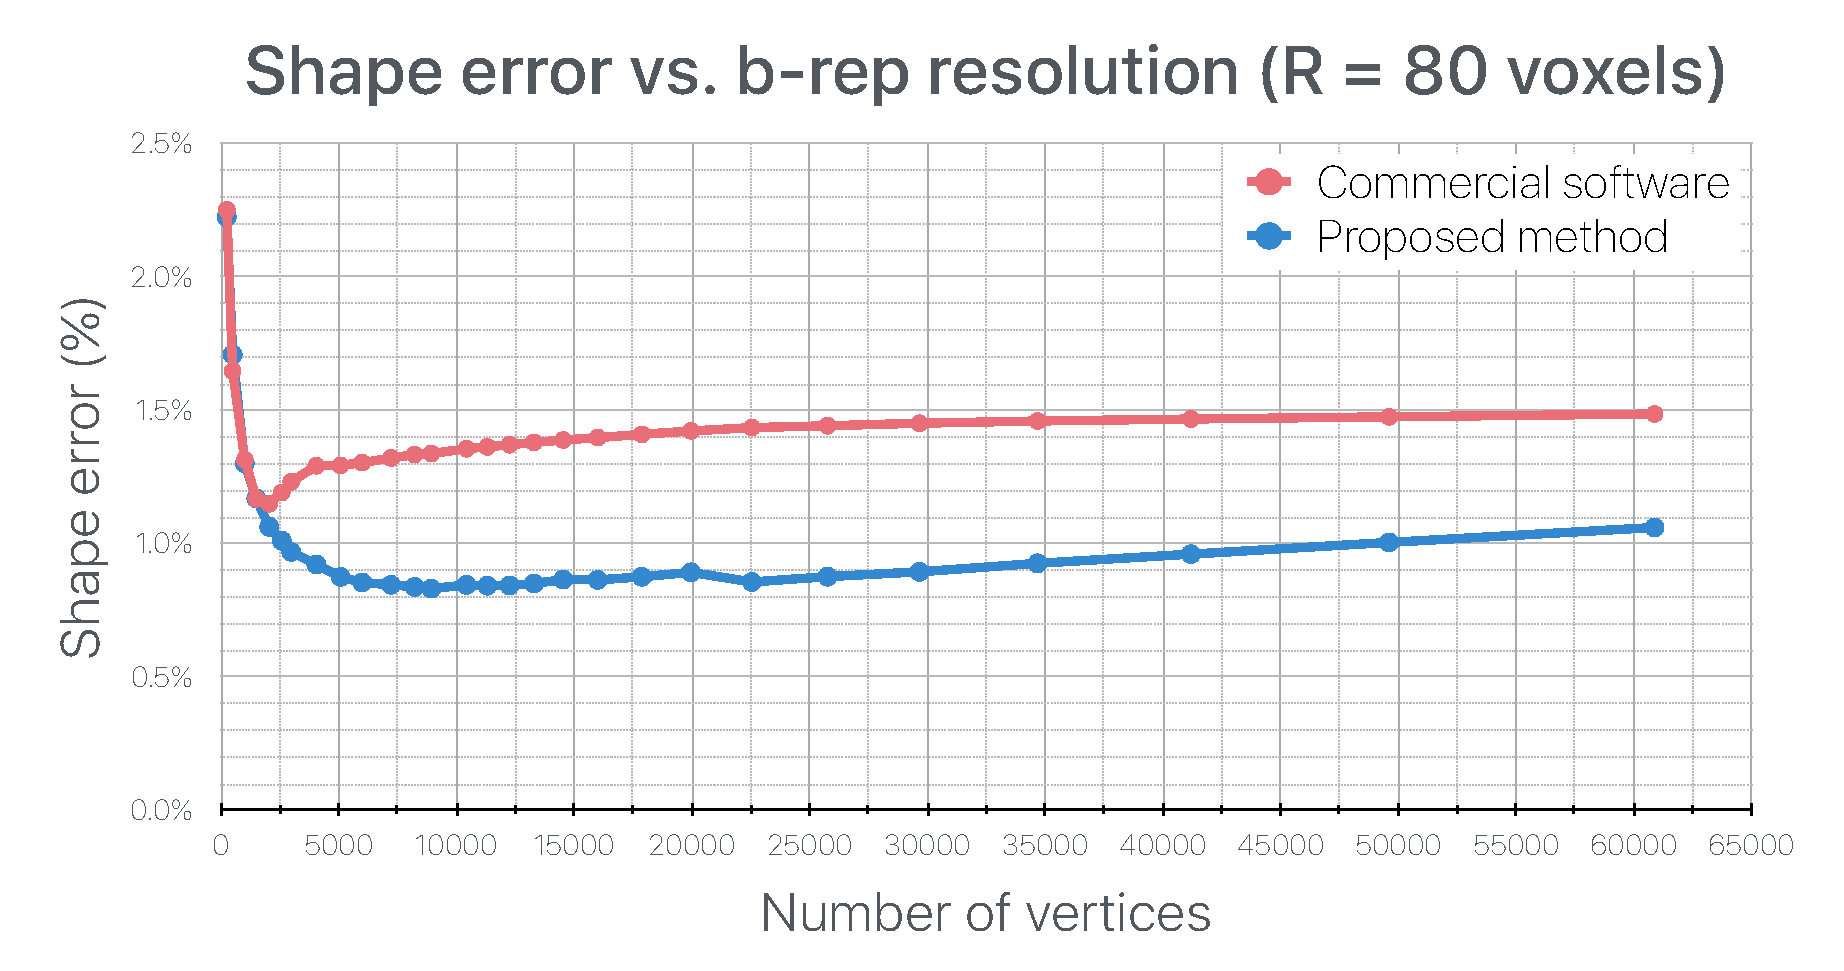
\includegraphics[scale=0.28]{media/7-performance/11-graph-1a.pdf}}
\subfigure[]{%
	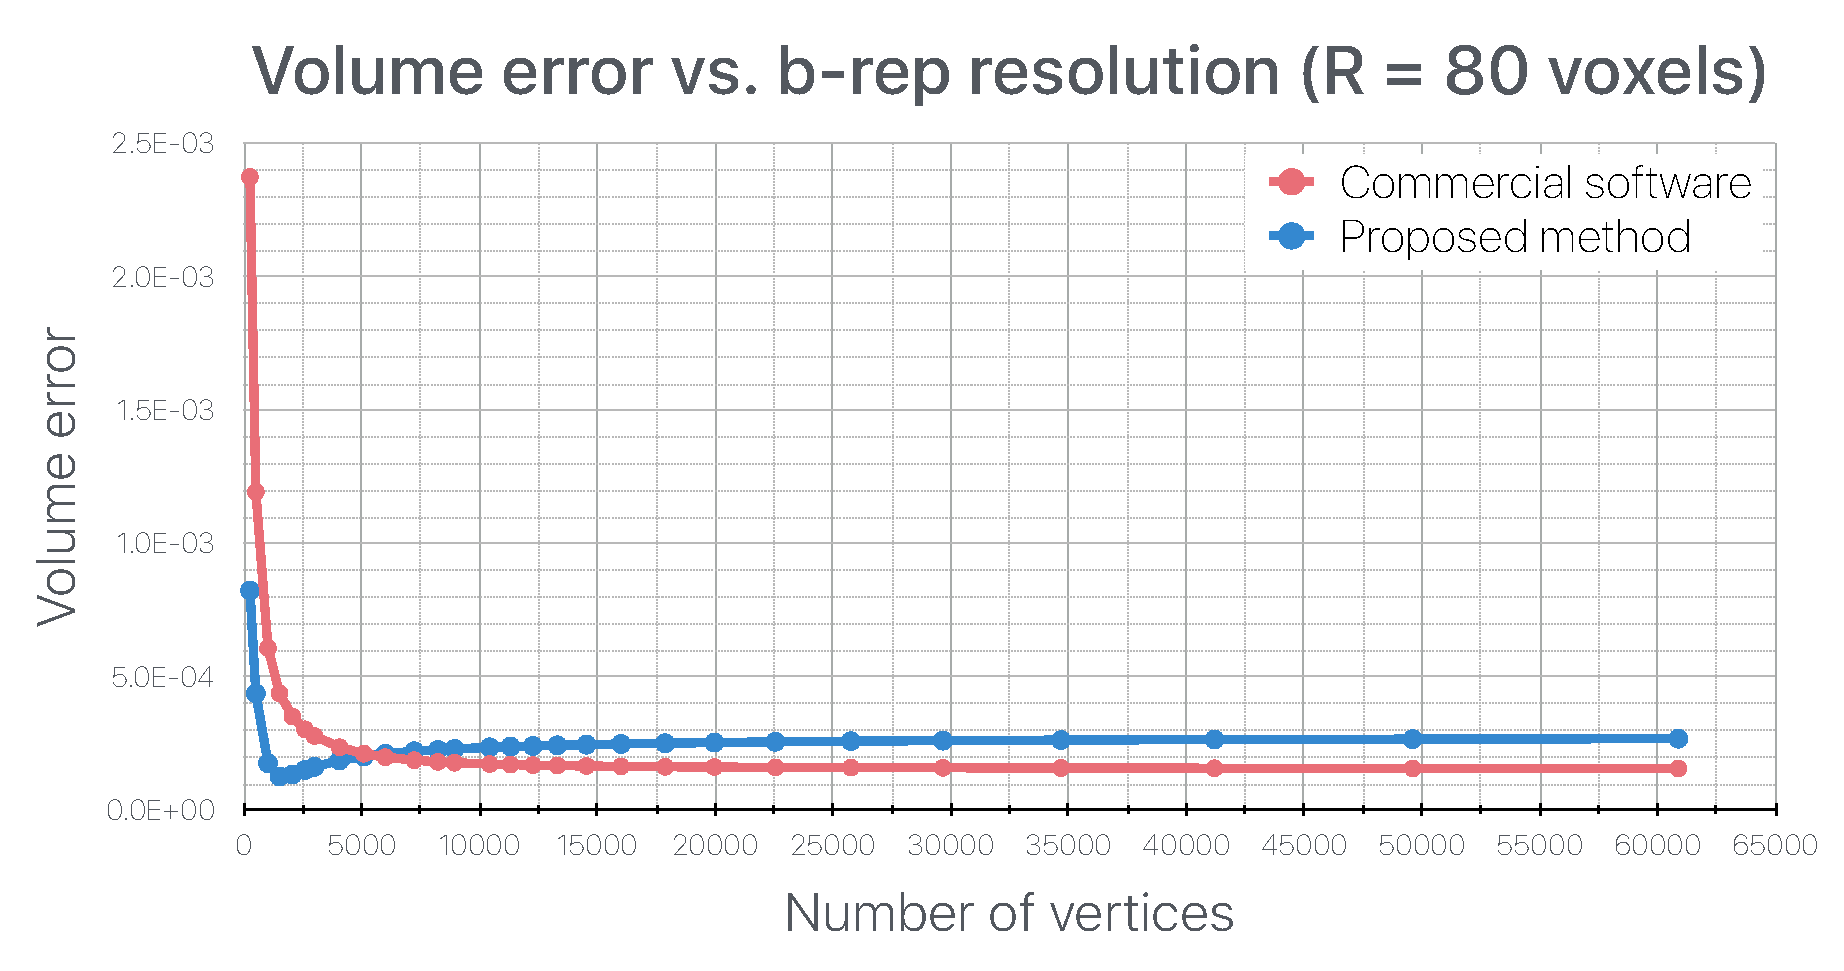
\includegraphics[scale=0.28]{media/7-performance/11-graph-1b.pdf}}
%	
\caption{Comparison of shape error (a) and volume error (b) between commercial software and proposed method as b-rep resolution is varied.}
\label{fig:graph1}
\end{figure}
\begin{figure}[ht!]
	\centering
	\includegraphics[scale=0.25]{media/7-performance/3-demos-4.pdf}
	\caption{Image masks (green) and corresponding b-reps for commercial software (red) and proposed method (blue) for selected b-rep resolutions.}
	\label{fig:demos1}
\end{figure} \\
%
\figref{graph2} shows the error metrics when the radius of the spherical mask is varied from 40 to 120 voxels, while keeping the sphere centered in the image and the b-rep resolution fixed at $n = 10428$ vertices. See~\figref{demos2} for representative examples of the image mask and resulting b-reps from the two methods. The sphere radius represents an inverse measure of the curvature of the image mask relative to the voxel resolution; larger radii correspond to smoother surfaces. Both the shape and volume errors of the proposed method converge at roughly double the rate of those of the commercial approach as the radius is increased. The proposed method's shape error is the smaller of the two over the entire range of sphere radii considered, while its volume error is the greater over most of the range of radii.

\begin{figure}[b!]
	\centering
	\subfigure[]{%
		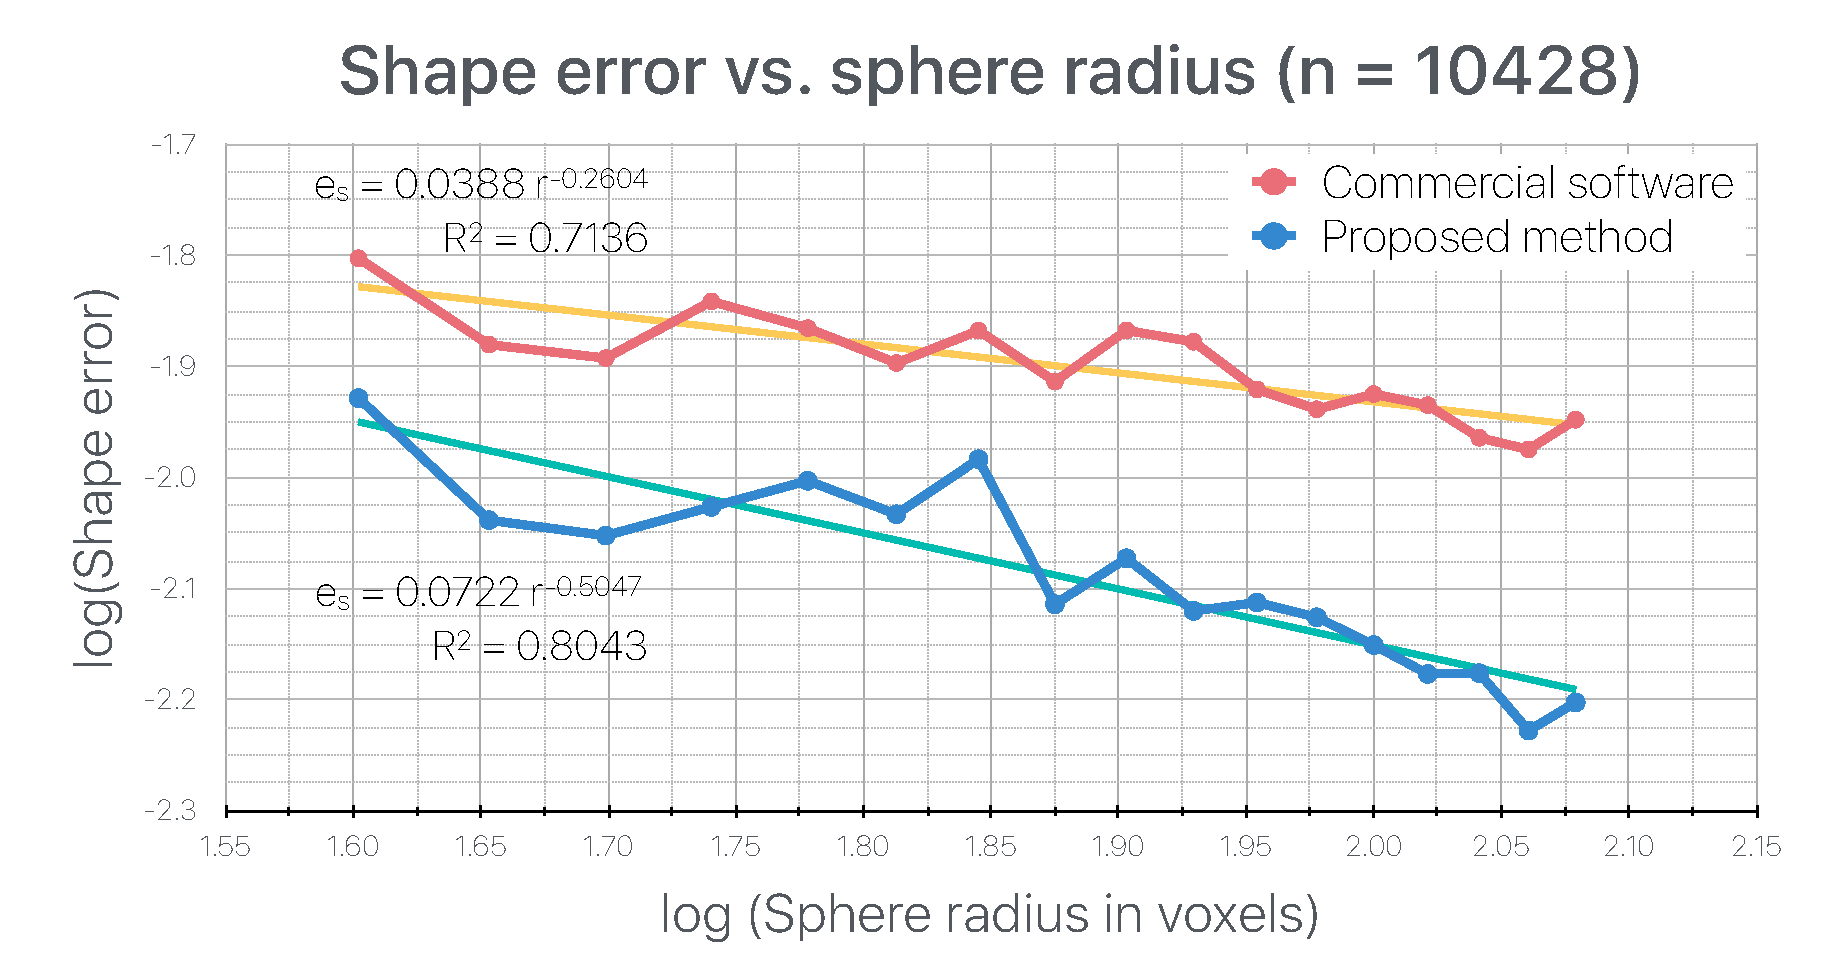
\includegraphics[scale=0.28]{media/7-performance/11-graph-2a.pdf}}
	\subfigure[]{%
		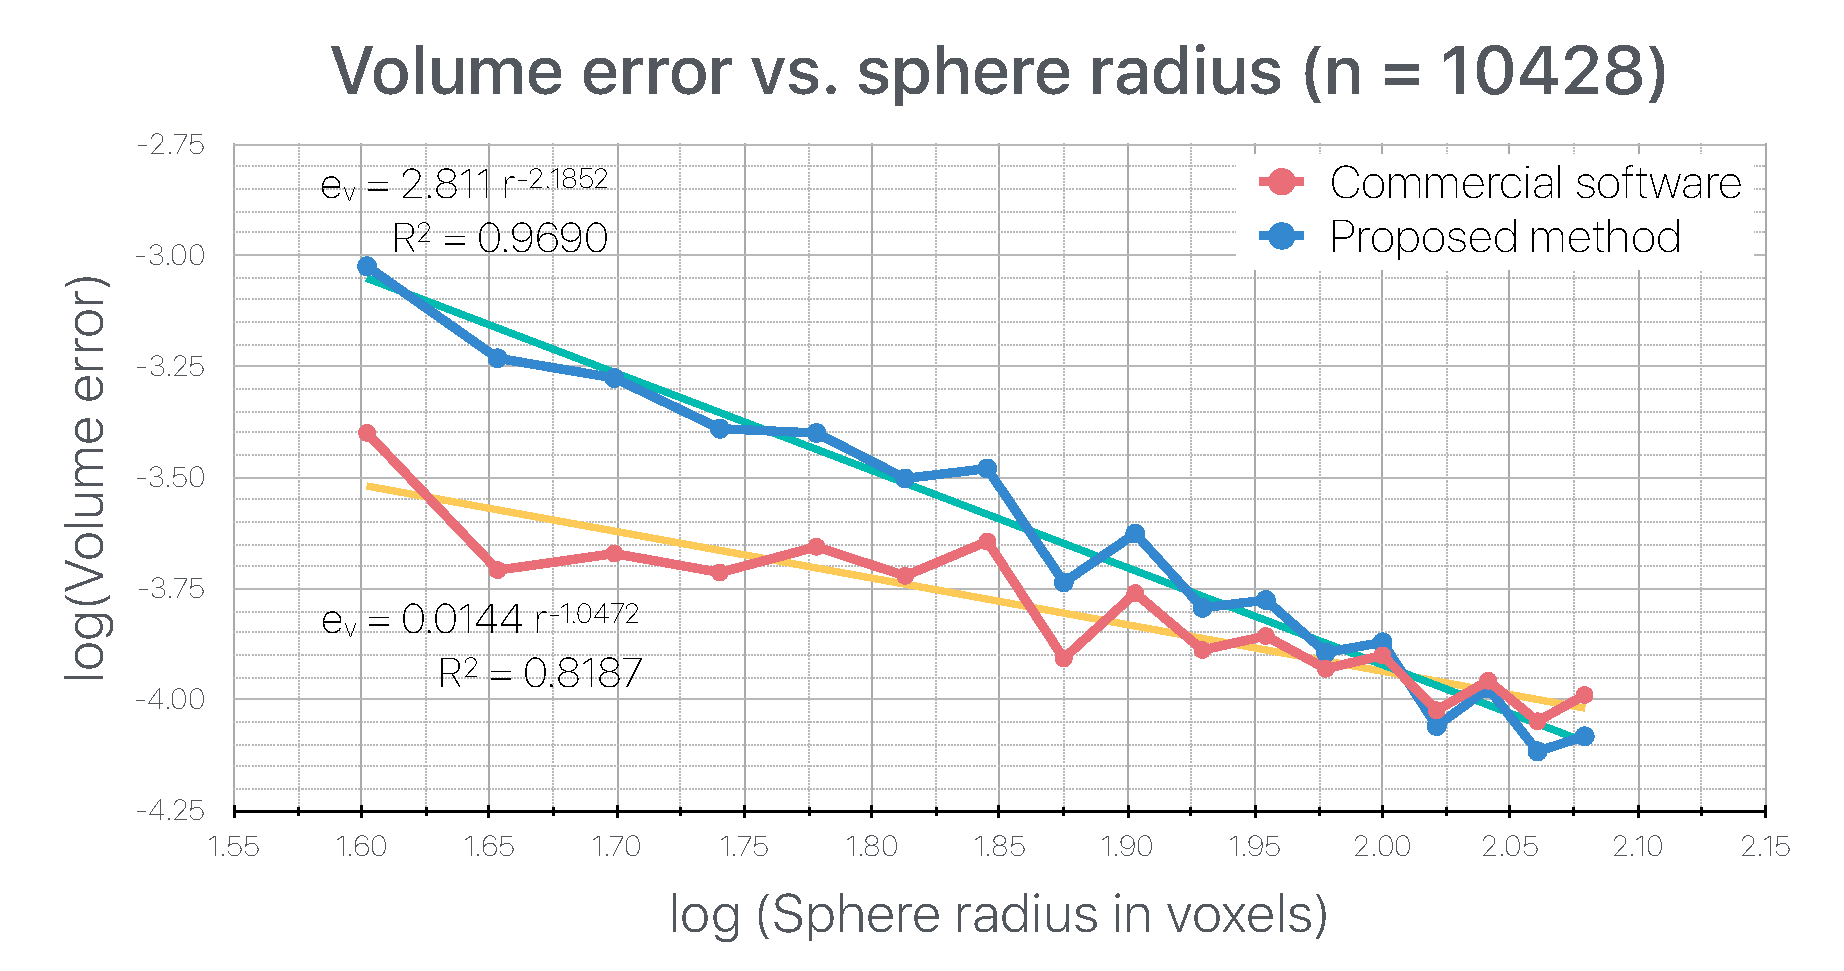
\includegraphics[scale=0.28]{media/7-performance/11-graph-2b.pdf}}
	%	
	\caption{Comparison of shape error (a) and volume error (b) between commercial software and proposed method as the radius of the exact sphere is varied.}
	\label{fig:graph2}
\end{figure}
\begin{figure}[ht!]
	\centering
	\includegraphics[scale=0.25]{media/7-performance/3-demos-5.pdf}
	\caption{Image masks (green) and corresponding b-reps for commercial software (red) and proposed method (blue) for selected sphere radii.}
	\label{fig:demos2}
\end{figure}
{\noindent}As a final point of quantitative comparison, the two methods are compared for a sphere of $R = 80$ voxels that is translated from center along the direction $\bm{i}  + 2\bm{j} + 3\bm{k}$, while keeping the resulting b-rep fixed at $n = 10428$ vertices. The intent of this case is to test the sensitivity of the methods to the location of the object relative to the image's voxel array. Ideally, the b-reps should be consistently accurate regardless of location.  Indeed, both methods show very low sensitivity to the translation of the object within the image, as shown in~\figref{graph3}. The relative standard deviations in shape error for the commercial software and proposed method were $2.4\%$ and $1.1\%$, respectively. For volume error, they were $1.7\%$ and $2.1\%$. \\

\begin{figure}[b!]
	\centering
	\subfigure[]{%
		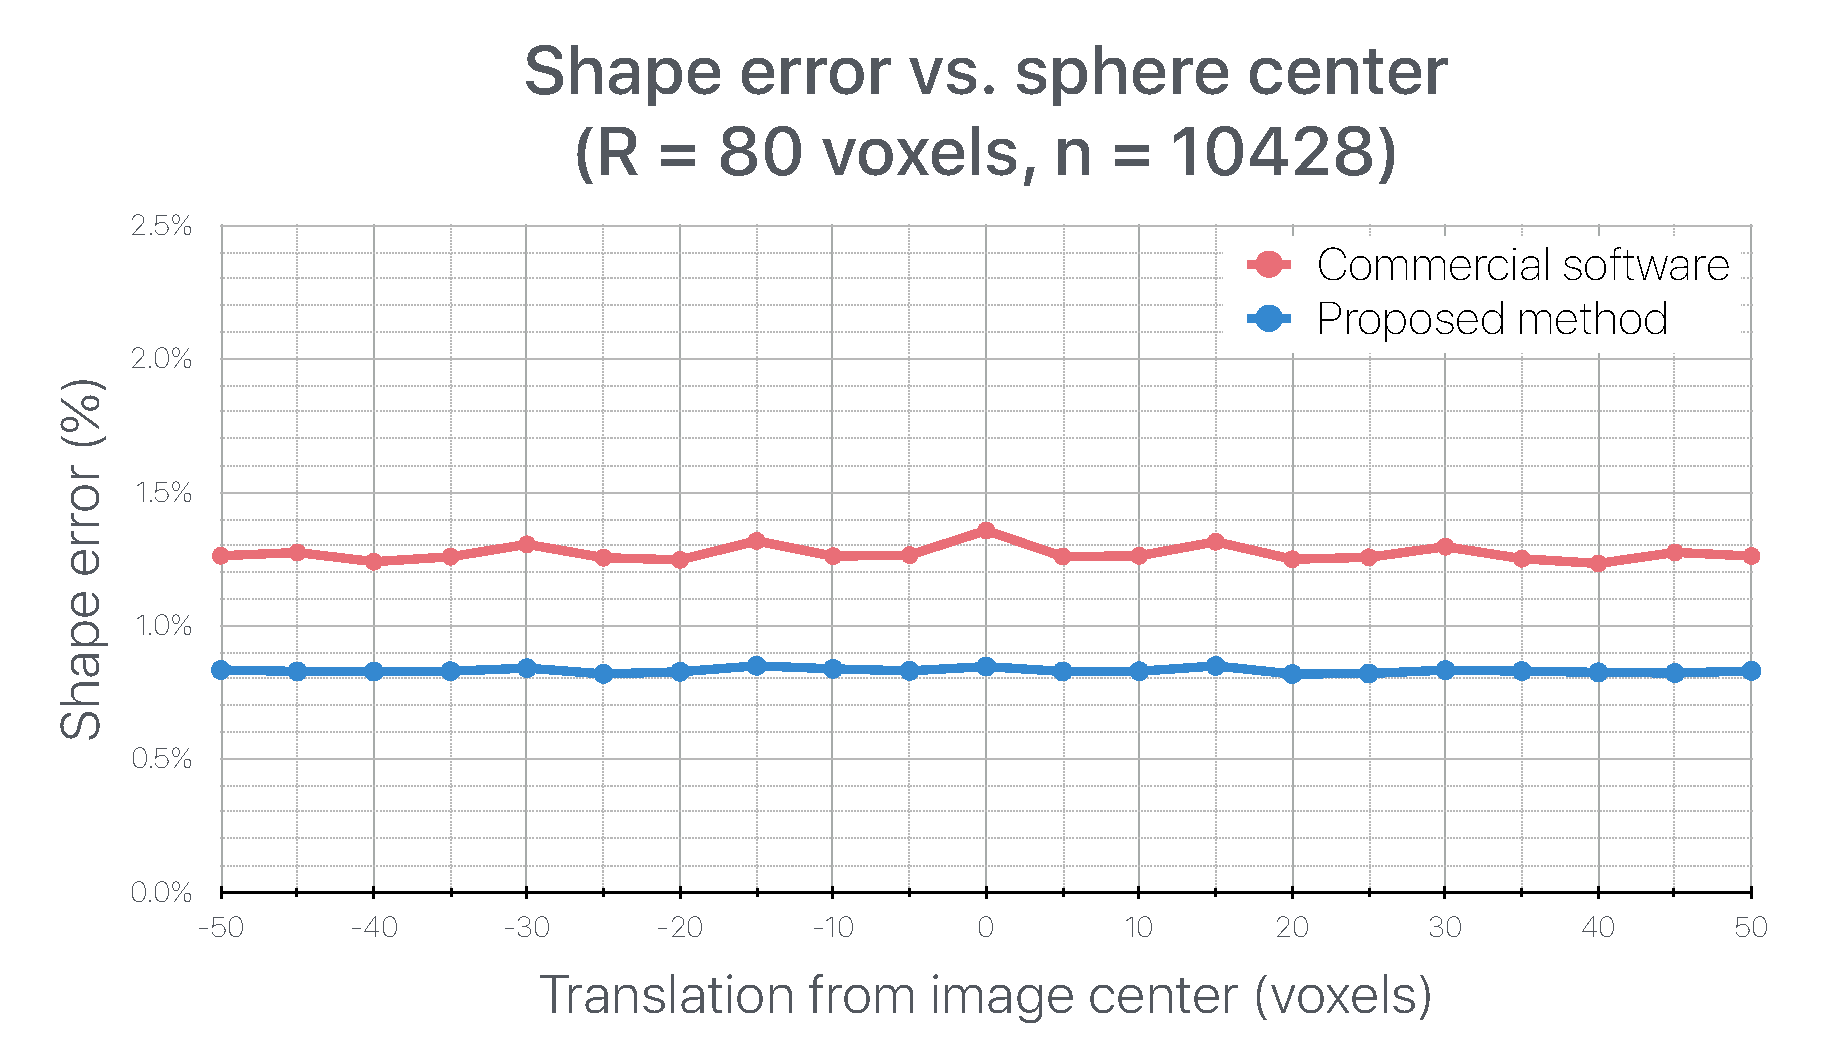
\includegraphics[scale=0.28]{media/7-performance/12-graph-3a.pdf}}
	\subfigure[]{%
		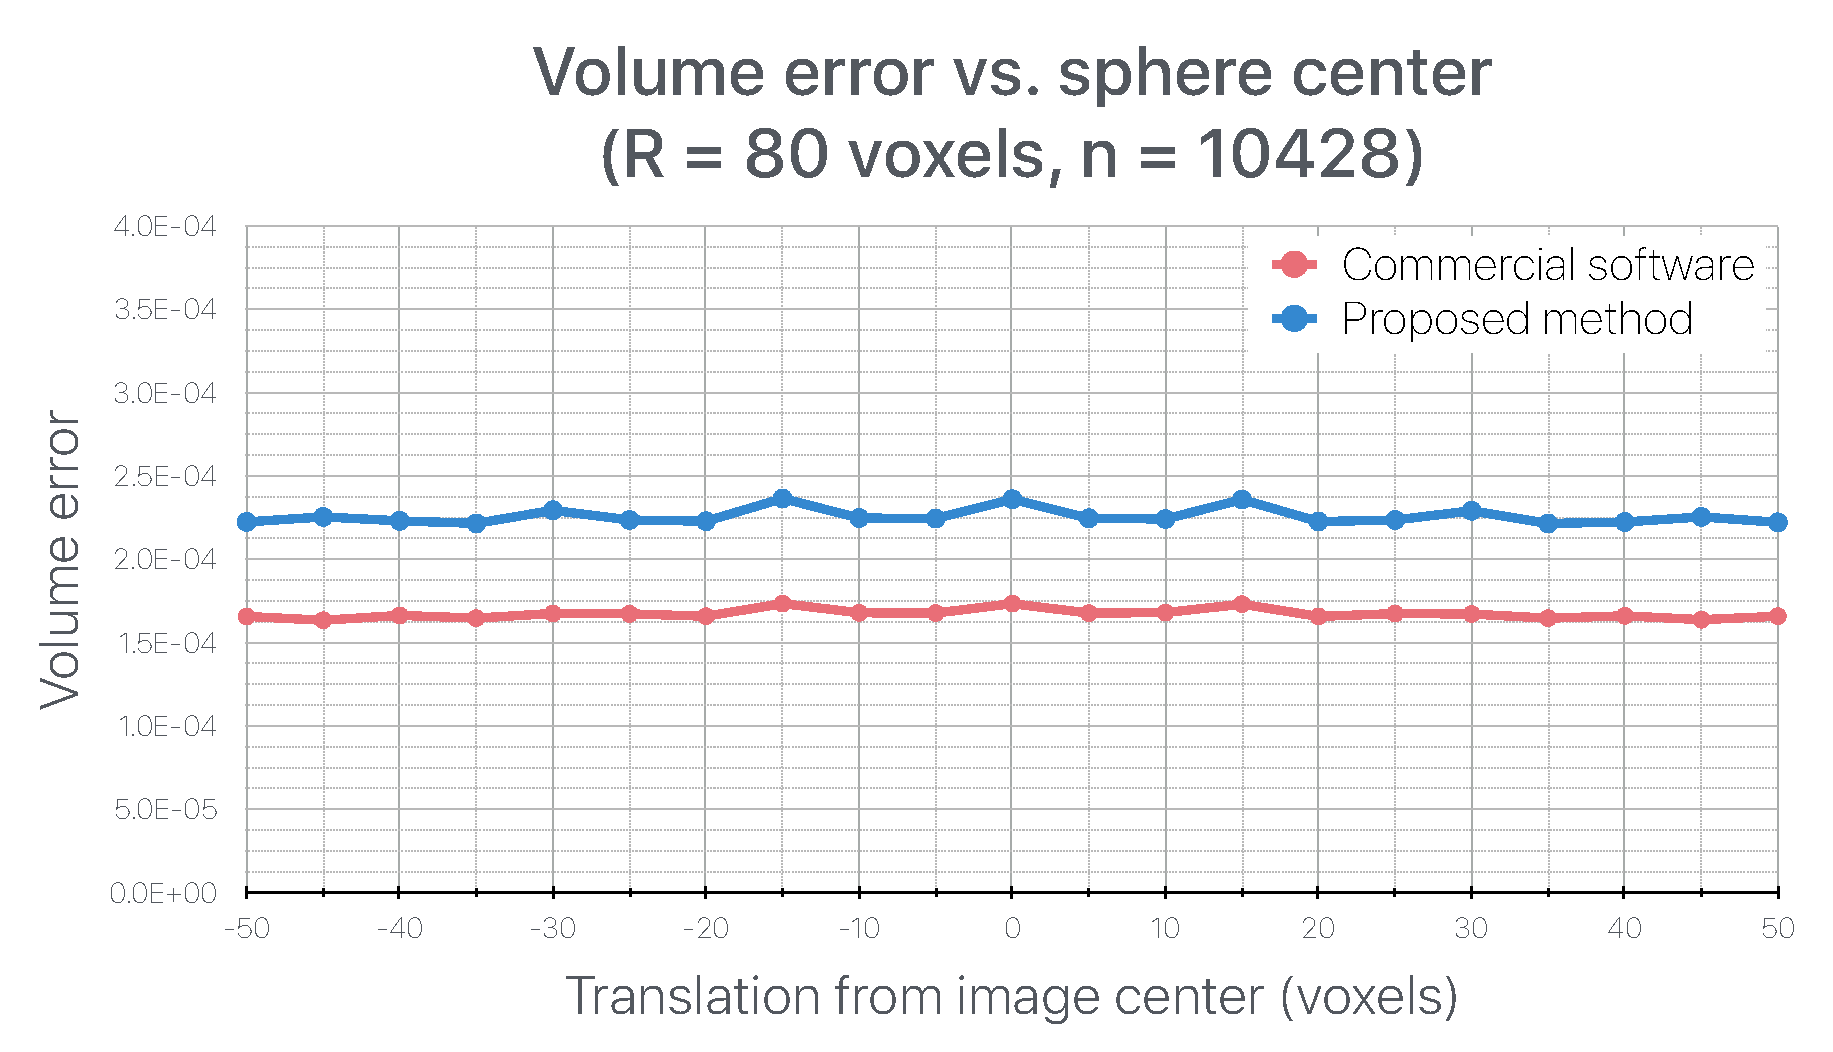
\includegraphics[scale=0.28]{media/7-performance/12-graph-3b.pdf}}
	%	
	\caption{Comparison of the shape error (a) and volume error (b) between the commercial software and the proposed method as the center of the sphere is translated relative to the image mask.}
	\label{fig:graph3}
\end{figure}
%%%%%%%%%%%%%%%%%%%%%%%%%%%%%%%%%%%%%%%%%%%%%%%
%%%%%%%%%%%%%%%%%%%%%%%%%%%%%%%%%%%%%%%%%%%%%%%
\subsection{\textcolor{purple}{The Polluted Sphere}}
\label{The Polluted Sphere}

\color{purple}

Text

\color{black}
%%%%%%%%%%%%%%%%%%%%%%%%%%%%%%%%%%%%%%%%%%%%%%%
%%%%%%%%%%%%%%%%%%%%%%%%%%%%%%%%%%%%%%%%%%%%%%%
\subsection{\textcolor{purple}{Complex Surfaces}}
\label{Complex Surfaces}

Lastly, we present several qualitative comparisons based on real image masks generated from MRI and CT.  All images were segmented using \textit{Seg3D}~\cite{Seg3D}. The resulting binary image masks were used as input to the two methods. B-rep resolutions were matched between the two approaches in all cases, to make for a fair comparison. All examples completed for the proposed method on a 16 GB RAM laptop in less than 5 minutes. See~\figref{example-meshes} for comparison of the image masks and resulting b-reps. Visual inspection suggests that the proposed method qualitatively performs comparably to the commercial approach in all cases, performing slightly better for smooth surfaces and not quite as well for regions with high curvature.  In this connection, we mention that the proposed method readily accommodates an enhancement that admits sharp edges and vertices (or corners), making the method particularly suitable for industrial applications involving manufactured objects.  Work on this enhancement is in progress.  The suite of examples presented here nonetheless show a robustness and quality that illustrate the proposed method as a viable approach as it stands.
\begin{figure}[h!]
	\centering
	\includegraphics[scale=0.08	]{media/7-performance/realExamples.pdf}
	\caption{Comparison of proposed method to existing approaches for various input image masks generated from MRI and CT scans. Note the proposed method's robustness to noisy inputs for the brain (upper right), distal femur (middle left), and equine proximal sesamoid (bottom right). The ``marching cubes'' approach applies the same decimation and smoothing as the proposed method following conventional marching cubes, for fair comparison. The ``Screened Poisson'' approach applies Screened Poisson surface reconstruction on oriented point clouds generated from the scheme described in the proposed method. Sources: heart~\cite{cvgg}, lungs~\cite{rikxoort_2009}, distal femur~\cite{epperson_2013}, liver~\cite{bilic_2019}, upper left second molar (author's), brain~\cite{marcus_2007}, skull~\cite{clark_2013}, pelvis~\cite{clark_2013}, L5 lumbar~\cite{yao_2016}, and equine proximal sesamoid~\cite{shaffer2021}}
	\label{fig:example-meshes}
\end{figure}